\documentclass[a4paper,12pt]{ctexart}

\usepackage{epsf,psfrag,graphicx,color}
\usepackage{hyperref,amssymb}
\usepackage{verbatim}
\usepackage{fancybox}
\usepackage{tcolorbox}

\newcommand{\mybox}[1]{\fcolorbox{black}{blue}{\parbox{\textwidth}{\color{white}#1%
}}}

\definecolor{mycolor}{rgb}{0.122, 0.435, 0.698}% Rule colour
\makeatletter
\newcommand{\myboxx}[1]{%
  \setbox0=\hbox{#1}%
  \setlength{\@tempdima}{\dimexpr\wd0+13pt}%
  \begin{tcolorbox}[colframe=mycolor,boxrule=0.5pt,arc=4pt,
      left=6pt,right=6pt,top=6pt,bottom=6pt,boxsep=0pt,width=\@tempdima]
    #1
  \end{tcolorbox}
}
\makeatother

\definecolor{bt}{rgb}{0.23, 0.55, 0.96}

\newtcbox{\myovalbox}{colback=bt,%
  fontupper=\footnotesize\sffamily\color{white},%
  boxrule=0pt,arc=5pt,%
  boxsep=2pt,left=3pt,right=3pt,top=3pt,bottom=3pt}%

% ctex + xelatex 下 \scshape 不可用（TU/lmr/bx/sc 未定义），会导致字体重叠与警告。
% 这里改用普通罗马字体并加粗，保持品牌名醒目即可。
\newcommand{\qchem}{\href{https://q-chem.com}{\textbf{Q-Chem}}}
\newcommand{\iqmol}{\href{https://www.iqmol.org}{\textbf{IQmol}}}
\newcommand{\symmol}{\textbf{Symmol}}

\newcommand{\heading}[1]{ \noindent{ \large \bf{#1} }}
\newcommand{\myline}{\setlength{\unitlength}{1mm}
                     \begin{picture}(160,2)
                     \put(0,0){\line(1,0){160}}
                     \put(0,1){\line(1,0){160}}
                     \end{picture}
                    }
\newcommand{\showlines}[1]{}

\newcommand{\alert}[1]{\textcolor{red}{#1}}
\newcommand{\sci}[2]{\ensuremath{#1\times 10^{-#2}}}
\newcommand{\mc}{\multicolumn}
\newcommand{\R}[1]{\ensuremath{\mathrm{#1}}}
\newcommand{\B}[1]{\ensuremath{\mathbf{#1}}}

\newcommand{\bt}{\ensuremath{\blacktriangleright}}
\newcommand{\ie}{\emph{即}}
\newcommand{\eg}{\emph{例如}}

\setlength{\headheight}{0cm}
\setlength{\topmargin}{1cm}
\setlength{\headsep}{0cm}
\setlength{\voffset}{0cm}
\setlength{\oddsidemargin}{0cm}
\setlength{\evensidemargin}{0cm}
\setlength{\hoffset}{0cm}

\setlength{\textheight}{23.0cm}
\setlength{\textwidth}{16cm}

\setlength{\parindent}{0cm}
\setlength{\parskip}{1em}
\setlength{\unitlength}{1mm}
\usepackage{chngcntr}
\counterwithin{figure}{section}

%----------------------------------------------------------------------%
\begin{document}
%----------------------------------------------------------------------%

\thispagestyle{empty}
\noindent
\myline\\
\begin{center}
{\bf \LARGE IQmol 使用简介}
\end{center}
\myline\\

\vfill

\begin{center}
\includegraphics[scale=0.25]{figures/Crown.png}
\end{center}

\vfill
%\myline\\
\begin{center}
{\large v3.2 (2025) Andrew Gilbert}
\end{center}
%\myline\\

\newpage

\tableofcontents

\newpage


%----------------------------------------------------------------------%
\section{简介}
%----------------------------------------------------------------------%

\iqmol{} 是一款开源的分子编辑与可视化软件，可运行于 Windows、Mac OS X 以及 Linux
系统。它能够读取多种化学文件格式，包括 xyz、cml、pdb、mol、fchk、cube 数据以及
\qchem{} 的输入/输出文件。软件还内置了一个自由形式的分子构建器，可用于创建任意分子结构。
这些结构可以利用分子力学力场进行优化，并通过对称化操作确保结构具有正确的点群对称性。
此外，软件提供一个分子库和官能团库，可用于辅助构建更复杂的分子。

\iqmol{} 能够显示多种分子性质，包括原子电荷、偶极矩和简正振动模式。它可以显示多种类型的
表面，包括分子轨道、（自旋）密度以及范德华表面。这些表面可以根据任意标量场（例如静电势）
进行着色。软件还支持振动频率、反应路径以及优化路径的动画演示。

\iqmol{} 可以作为独立软件包使用，同时也被设计为与 \qchem{}（\url{https://www.q-chem.com}）
计算化学程序包无缝配合工作。其内置的综合性输入文件生成器——\qchem{} 用户界面（QUI）——
提供了对 \qchem{} 中绝大多数可用选项的访问，并以直观的分层方式呈现这些选项。所生成的输入文件
可以提交到本地或远程服务器上运行，只要目标服务器已安装 \qchem{} 软件即可。特别地，\iqmol{}
提供了一个公共可访问的服务器，允许用户在不购买和安装 \qchem{} 的情况下运行有限时长（约 10 分钟）
的量子化学计算。



\subsection{安装}

\iqmol{} 的最新版本可从官方网站下载：
\vspace{-1.0em}
\begin{center}
\url{https://www.iqmol.org/downloads.html}
\end{center}
\vspace{-1.0em}

对于 Mac（OS X）系统，提供磁盘映像文件。下载后，双击磁盘映像将其挂载，并将应用程序复制到
Applications 目录或任何其他期望的位置即可。

对于 Windows 系统，提供安装程序，它将引导您完成安装过程，并在桌面上创建程序的快捷方式。

对于 Linux 系统，现已提供 .deb 和 .rpm 软件包，可分别使用 dpkg 或 yum 进行安装：

\hspace*{2em}{\tt \#>  sudo dpkg -i iqmol\_x.x.x.deb}\\
\hspace*{2em}{\tt \#> sudo apt-get install -f }

第二条命令用于解决对 Qt 库的依赖关系，您可能尚未安装该库。

\hspace*{2em}{\tt \#>  sudo yum install iqmol-x.x.x.x86\_64.rpm}

请注意，无论哪种情况，您都需要具有 root 权限。


\subsection{概览}
\label{sec:overview}

\begin{figure}[ht]
\begin{center}
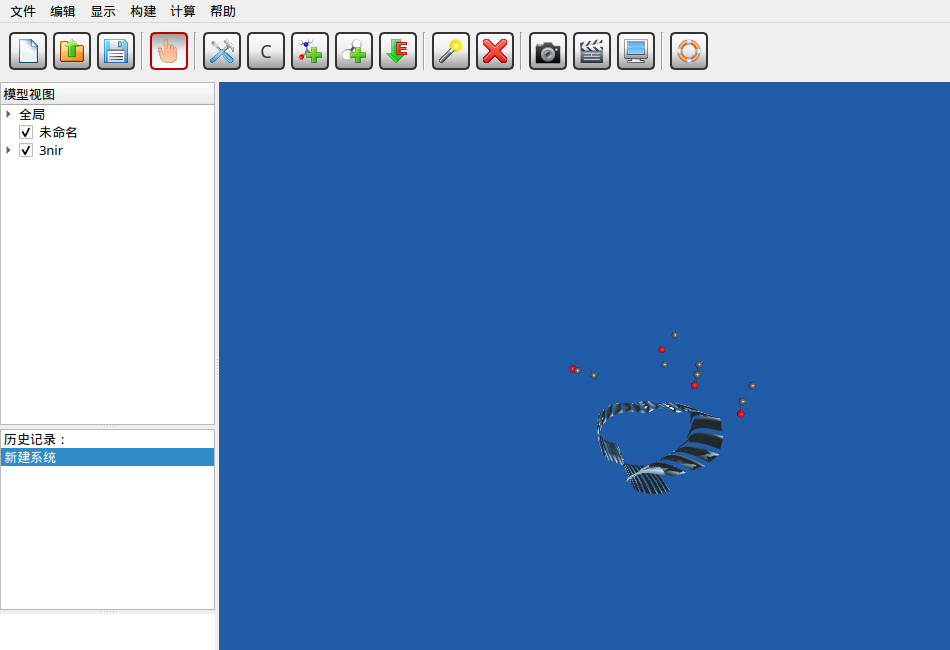
\includegraphics[scale=0.35]{figures/Viewer.png}
\caption{\iqmol{} 的主窗口。}
\label{fig:main}
\end{center}
\end{figure}
\iqmol{} 的主窗口如图~\ref{fig:main} 所示，由以下几个主要部分组成：
\begin{itemize}
\item {\bf 查看器（Viewer）}是窗口的主要区域，您可以在其中查看并与分子进行交互。
\item 顶部的 {\bf 工具栏（Toolbar）}提供对常用命令的访问，并允许在不同查看器模式之间切换，
      包括操纵模式
      \includegraphics[scale=0.40]{figures/ManipulateButton.png}、选择模式
      \includegraphics[scale=0.40]{figures/SelectButton.png} 以及构建模式。
      \includegraphics[scale=0.40]{figures/BuildButton.png}
\item {\bf 模型视图（Model View）}面板以分层方式展示分子可用的数据。
\item 左下角的 {\bf 历史（History）}面板列出了最近的操作，可以通过单击这些操作或使用
      编辑 \bt\ 撤销菜单项来撤销它们。
\end{itemize}

模型视图（MV）控制查看器中显示哪些对象，并允许访问这些对象的配置选项。可见性由相应的
复选框控制。取消勾选复选框会使该项及其所有子项都被隐藏。如果某项没有复选框（例如化学键），
则其可见性只能由层级中更高层级的项来控制。

许多对象的外观可以通过在模型视图中双击该项进行配置。例如，双击分子名称会弹出
"配置分子"对话框，允许您更改分子结构的显示外观：
\begin{center}

\includegraphics[scale=0.25]{figures/MoleculeConfigurator.png}
\end{center}
请注意，可以在同一个查看器中同时显示多个分子，并且每个分子的外观都可以单独配置。
\begin{figure}[h]
\begin{center}
\includegraphics[scale=0.18]{figures/CHF3-balls.png}\hspace{-3mm}~
\includegraphics[scale=0.20]{figures/CHF3-wire.png}\hspace{-3mm}~
\includegraphics[scale=0.18]{figures/CHF3-space.png}\hspace{-3mm}~
\includegraphics[scale=0.18]{figures/CHF3-tubes.png}\hspace{-3mm}~
\includegraphics[scale=0.18]{figures/CHF3-moly.png}
\caption{分子结构的渲染样式：球棍模型、线框模型、空间填充模型、管状模型以及塑料模型。}
\label{fig:styles}
\end{center}
\end{figure}


%----------------------------------------------------------------------%
\newpage
\section{构建分子}
%----------------------------------------------------------------------%


\subsection{添加原子与片段}


默认情况下，\iqmol{} 以构建模式打开。这由工具栏中
\includegraphics[scale=0.40]{figures/BuildButton.png} 按钮周围的红色边框指示。当前构建的
默认原子由
\includegraphics[scale=0.40]{figures/BuildAtomButton.png} 按钮指示，单击该按钮可以更改它。
将弹出一个周期表窗口，从中可以选择所需的元素类型。

在空白的查看器窗口中单击将创建一个当前构建元素的原子。通过单击现有原子并拖动鼠标可以添加
更多原子，这会创建一个与第一个原子成键的新原子。要创建不相连的原子，请在单击查看器窗口时
按住 \emph{alt} 修饰键。（请注意，某些 Linux 窗口管理器将 \emph{alt} 修饰键用于其他用途。
此行为可以通过"系统设置 \bt\ 键盘 \bt\ 快捷键"菜单进行更改。）

通过单击并拖动两个现有原子之间可以增加键级。如果两个原子之间不存在键，则会创建一条键；
否则键级会增加。要降低键级，必须首先删除该键，然后创建一个新键。
\begin{figure}[h]
\begin{center}
\includegraphics[scale=0.25]{figures/Cdouble.png}
\caption{增加键级。}
\end{center}
\end{figure}


可以通过单击
\includegraphics[scale=0.40]{figures/BuildFragButton.png} 按钮、确保"官能团"单选按钮被选中并从
菜单中选择所需的基团来添加官能团。基团的添加方式与原子相同，\emph{即}从现有原子单击并拖动。
空的价键由黄色键指示，并显示基团将连接的位置。
\begin{figure}
\begin{center}
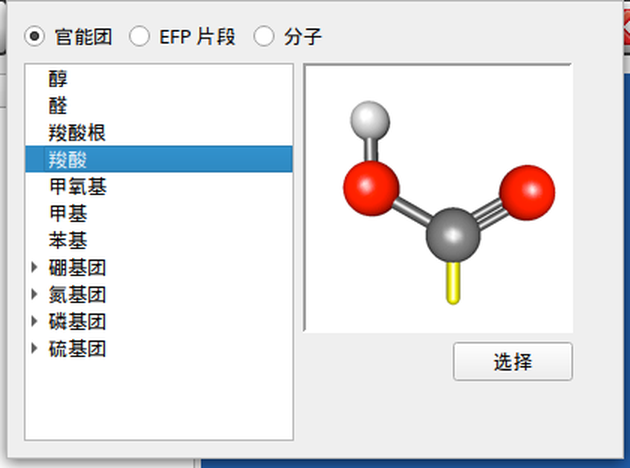
\includegraphics[scale=0.5]{figures/FunctionalGroup.png}
\caption{单击添加片段按钮时出现的构建片段弹出窗口。}
\end{center}
\end{figure}


也可以通过单击
\includegraphics[scale=0.40]{figures/BuildFragButton.png} 按钮、确保"分子"单选按钮被选中并从菜单中
选择所需的分子，将整个分子添加到您的系统中。请务必单击 \Ovalbox{选择}，否则构建选择不会被更新。
与其他构建模式不同，在查看器窗口中任何位置单击都会添加所选分子（不需要鼠标修饰键）。这样可以
快速添加多个相同类型的分子（\eg\ 用于溶剂化），但会改变通常的鼠标行为。如果您不小心添加了过多
分子，请使用编辑 \bt\ 撤销菜单项。添加分子时，如果单击并按住，可以在将新添加的分子加入全局
坐标系之前改变其局部取向。
%\begin{center}
%\includegraphics[scale=0.5]{figures/BuildMol.png}
%\end{center}

一旦分子的骨架绘制完成，可以单击添加氢原子按钮
\includegraphics[scale=0.40]{figures/AddHydrogensButton.png} 来自动向任何未填满的价键添加氢原子。
该操作会根据每个原子当前的化合价推断应补充的氢数目，对于绝大多数有机分子都能得到正确的加氢原子结果。
如果某些原子希望保持不饱和（例如用于后续手动成键），可在添加氢原子之前先调整相关原子的价态，或在
添加后手动删除多余的氢。

\paragraph{实用提示}
\begin{itemize}
\item 添加氢原子应在完成骨架绘制、且尚未进行对称化之前进行，这样对称化操作才能一并处理新加入的氢。
\item 若绘制时误加了多余原子，使用编辑 \bt\ 撤销（或历史面板）即可回退到上一步，无需手动删除。
\item 对于带电体系或含有金属原子的结构，自动加氢可能不准确，建议结合检查点文件中的实际结构进行核对。
\end{itemize}



\subsection{利用分子力学优化结构}

\iqmol{} 中的构建器是自由形式的，因此您的初始结构可能看起来有些怪异。要改善几何结构，请单击
\includegraphics[scale=0.40]{figures/MinimizeEnergyButton.png} 按钮。这将使用分子力学（MM）力场
优化几何结构。默认力场是通用力场（UFF）\cite{UFF}，其优点是几乎为整个周期表所定义。然而，UFF 对于
含有氢键的体系表现不佳，在这种情况下，建议使用构建 \bt\ 选择力场菜单项更改力场。

\begin{figure}[h]
\begin{center}
\includegraphics[scale=0.5]{figures/ForceFieldMenu.png}
\caption{更改分子力学力场。}
\end{center}
\end{figure}


\subsection{对称化结构}

如果您的分子具有对称性，分子力学优化不太可能找到具有所需对称性的结构。在这种情况下，可以使用
构建 \bt\ 对称化分子菜单项对接近对称的结构进行对称化。寻找非常高的对称性可能需要通过构建 \bt\
设置对称公差菜单项放宽公差。放宽公差允许程序移动更多核坐标，以便找到对称结构。

\iqmol{} 使用由 Tullio Pilati 和 Alessandra Forni 编写的 \symmol{}\cite{SymMol} 程序的修改版本来
对分子结构进行对称化。


\subsection{指定几何参数}

可以通过首先选择涉及的原子并使用构建 \bt\ 设置几何约束菜单项来设置几何参数的特定值。将弹出一个
对话框，允许将该参数设置为固定值、约束或扫描。约束参数适用于任何后续的分子力学优化，并且如果
请求了优化作业，还会传递到 \qchem{} 输入文件中。扫描选项也会传递到 \qchem{} 用于扫描作业。

\begin{figure}[h]
\begin{center}

\includegraphics[scale=0.5]{figures/ConstraintDialog.png}
\caption{用于设置几何约束的对话框}
\end{center}
\end{figure}

约束的类型取决于所选原子的数量：
\vspace{-1em}
\begin{enumerate}
\itemsep0em
\item 固定原子位置
\item 原子间距离（或选择单条化学键）
\item 键角
\item 扭转（二面角）角
\end{enumerate}
活动约束在查看器中可见，可以通过单击模型视图中相邻的复选框来停用它们。


\subsection{操纵与选择分子}
\label{sec:mousemodes}

\iqmol{} 设计用于与三键鼠标或触控板配合使用效果最佳。如果您在 Mac 上使用触控板，建议通过
"系统偏好设置 \bt\ 触控板"启用辅助点击。

单击工具栏中的
\includegraphics[scale=0.40]{figures/ManipulateButton.png} 按钮可激活操纵模式，并实现以下鼠标功能：
\begin{itemize}
\item {\bf 左键单击并拖动：} 旋转分子的视图。
\item {\bf 中键单击并拖动：} 放大和缩小。
\item {\bf 右键单击并拖动：} 平移分子的视图。
\end{itemize}

也可以独立于其余部分操纵分子的某一部分。为此，请先创建选择，然后按住 \emph{ctrl} 修饰键
（在 Mac 上为 \emph{command} 键）。鼠标移动将仅影响所选原子，如下所示：
\begin{itemize}
\item {\bf 左键单击并拖动：} 绕其中心旋转所选原子。
\item {\bf 右键单击并拖动：} 平移所选原子。
\end{itemize}
如果只选择了单条化学键，则鼠标移动具有以下效果：
\begin{itemize}
\item {\bf 左键单击并拖动：} 绕键轴旋转。
\item {\bf 右键单击并拖动：} 改变键的长度。
\end{itemize}

单击工具栏中的
\includegraphics[scale=0.40]{figures/SelectButton.png} 按钮可激活选择模式，并实现以下鼠标功能：
\begin{itemize}
\item {\bf 左键单击：} 将原子或化学键添加到选择中。
\item {\bf 单击并拖动：} 创建选择矩形，选择矩形内的所有原子和化学键都被添加到选择中。
\item {\bf 右键单击：} 从选择中移除原子或化学键。
\end{itemize}
也可以通过编辑菜单下的选项来选择全部、选择无以及反转选择。


\subsection{添加额外的构象}

对于使用冻结字符串方法（FSM）设置作业，需要两个构象，分别对应字符串的初始和最终几何结构。
构建第一个几何结构后，可以通过在模型视图中右键单击分子名称来将第二个几何结构添加到分子中。
这将弹出一个带有"复制几何结构"选项的上下文菜单。
\begin{figure}[h]
\begin{center}
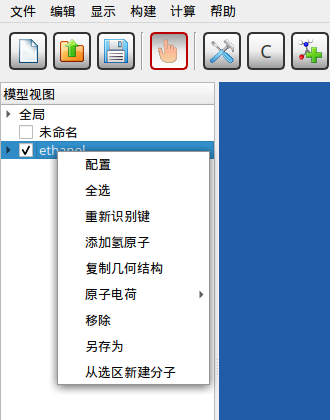
\includegraphics[scale=0.4]{figures/MoleculeContext.png}
\end{center}
\end{figure}
选择此菜单项会在模型视图中创建一个包含两（相同）个几何结构的"几何结构"项。可以通过在模型视图中
选择第二个几何结构并使用 \emph{ctrl}（在 Mac 上为 \emph{command}）修饰键在查看器中操纵所选原子来
修改它。如果在 QUI 中为计算选项选择"冻结字符串"（见下一节），则两个几何结构都将包含在输入文件的
\$molecule 部分中，以 **** 分隔。



%----------------------------------------------------------------------%
\newpage
\section{运行 \qchem{} 计算}
%----------------------------------------------------------------------%

\subsection{QUI}

\iqmol{} 内置了一个用于 \qchem{} 计算的输入文件生成器，即 QUI，可通过计算 \bt\ Q-Chem 设置菜单访问。
\begin{figure}[h]
\begin{center}

\includegraphics[scale=0.4]{figures/QUI.png}
\caption{\qchem{} 用户界面（QUI）对话框。}
\end{center}
\end{figure}

QUI 对话框的左侧包含用于设置计算的控件。这些控件以分层方式呈现，最常用的选项显示在面板顶部，
其他相关选项根据所选作业类型出现在下部区域。可以通过"高级"选项卡访问更高级的选项。生成的输入文件
显示在 QUI 右侧的面板中。

使用 QUI 设置一次计算的典型步骤如下：

\begin{enumerate}
\item {\bf 选择作业类型：} 在左侧面板的顶部选择计算类型，例如单点能（SP）、几何优化（OPT）、
      频率（FREQ）、过渡态搜索（TS）或各种更高阶的性质计算。选择后，面板会根据作业类型自动展开
      相关的选项组。
\item {\bf 设置计算方法：} 指定交换关联泛函（如 B3LYP、ωB97X-D）和基组（如 6-31G*、cc-pVTZ）。常用组合
      可直接从下拉列表中选择，非常用的可在"高级"选项卡中手动输入 \verb|$rem| 变量。
\item {\bf 指定分子与电荷/自旋多重度：} 分子取自当前查看器中的体系；若需要，可在输入中调整电荷与自旋
      多重度。若之前在构建阶段添加了多个构象（见"添加额外的构象"），并可在此选择"冻结字符串"等
      特殊计算模式。
\item {\bf 检查输入预览：} 对话框右侧实时显示生成的 \qchem{} 输入文件，建议在提交前核对 \verb|$molecule|、
      \verb|$rem| 与 \verb|$end| 段落是否正确。
\item {\bf 提交：} 单击"提交"按钮，在弹出的服务器列表中选择目标服务器，作业即在所选服务器上启动。
\end{enumerate}

若需要更精细的控制（例如自定义 DFT 色散校正、冻核近似、CC 相关方法选项等），请切换到"高级"选项卡。
在该选项卡中可以直接编辑 \verb|$rem| 段落，所有修改都会同步反映到右侧的输入预览中。

单击"提交"按钮将在所选服务器上启动作业。作业完成后，系统会提示您复制结果（对于远程服务器），然后
结果会自动加载到 \iqmol{} 中。当分子已用计算结果更新时，\includegraphics[scale=0.6]{figures/Favourites.png}
图标会出现在模型视图中分子名称的旁边。


\subsection{任务监视器}

已提交的作业可以通过计算 \bt\ 任务监视器菜单项进行监控。这将弹出任务监视器对话框，提供作业进度
信息。在任务监视器中右键单击某一行会弹出一个上下文菜单，允许终止或查询正在运行的作业，以及打开
已完成的作业。
\begin{figure}
\begin{center}

\includegraphics[scale=0.5]{figures/JobMonitor.png}
\caption{任务监视器对话框。右键单击所选作业会弹出一个带有附加选项的上下文菜单。}
\end{center}
\end{figure}

如果作业状态为错误，将鼠标悬停在状态上会显示错误消息。或者，双击作业将打开输出文件（如果可用），
并可能提供有关作业失败原因的额外信息。双击已完成的作业将从服务器复制结果（如果尚未复制）并重新
加载到主 \iqmol{} 窗口中。


\subsection{配置服务器}

默认情况下，\iqmol{} 配置为向位于加利福尼亚州普莱森顿的 \qchem{} 服务器提交作业。这是一个公共可访问的
服务器，任何希望在购买 \qchem{} 软件之前运行测试计算的人都可以使用。提交到此服务器的作业可以访问
\qchem{} 中可用的全套电子结构方法，但时间限制为 10 分钟。

可以配置其他服务器以访问已安装 \qchem{} 软件的其他计算机。这些计算机可以是本地服务器（\emph{即} 与运行
\iqmol{} 的机器相同），也可以是通过 SSH 连接的远程服务器。要添加其他服务器，请转到计算 \bt\ 编辑服务器
菜单项并单击 \includegraphics[scale=0.40]{figures/PlusButton.png} 按钮。
\begin{figure}
\begin{center}

\includegraphics[scale=0.5]{figures/ServerDialog.png}
\caption{服务器配置对话框。}
\end{center}
\end{figure}

配置服务器所需的信息取决于其类型，但每种情况都有默认选项。以下列出了应当考虑的最低要求：

\begin{itemize}
\itemsep0em
\item {\bf 本地：} 除非您确定机器上正在运行排队软件，否则将队列系统设置为"基本"。请确保在运行文件模板中
      （通过单击"配置"按钮访问）将 {\tt QC} 和 {\tt QCSCRATCH} 变量设置为正确的值。
\item {\bf SSH：} 需要通过 SSH 连接的目标机器的主机名和账户。除非您已设置替代的身份验证协议，否则请将
      身份验证组合框设置为"密码提示"。根据目标主机的设置方式，运行文件模板可能需要一些编辑才能正常工作，
      但这会因机器而异。
\item {\bf HTTP：} 默认选项应该适用。请注意，在 Windows 上应使用 HTTP（并且在 v2.8 中为默认），而对于 Mac 和
      Linux 可以使用 HTTPS，并且在未来版本中将成为默认。
\end{itemize}

% 导出和加载服务器配置


%----------------------------------------------------------------------%
\newpage
\section{分析结果}
\label{sec:anal}
%----------------------------------------------------------------------%


\iqmol{} 可以读取多种文件类型，并允许用户可视化其中包含的许多结果。可以通过文件 \bt\ 打开菜单项打开
单个文件，或者将文件拖放到查看器窗口中。也可以通过文件 \bt\ 打开目录菜单项打开目录，或者将目录拖放
到查看器上。

\iqmol{} 最常读取的结果文件类型包括：

\begin{itemize}
\itemsep0em
\item {\bf .out / .inp}：\qchem{} 的输出与输入文件，包含作业类型、能量、频率、轨道等信息。
\item {\bf .fchk}：格式化检查点文件，是绘制分子轨道与（自旋）密度的主要数据来源（GUI rem 变量需设为 2）。
\item {\bf .cube}：体数据文件，可包含电子密度、分子轨道或静电势，用于快速绘制等值面。
\item {\bf .xyz}：坐标文件，常用于读入反应路径或动画帧序列。
\item {\bf .pdb / .cml / .mol}：常见的分子结构格式。
\end{itemize}

将相关文件放在同一目录并通过"打开目录"一次性载入，可以避免基名不匹配导致部分数据未被关联的问题。

打开目录允许将与分子关联的多个文件一起加载，例如 \qchem{} 输出文件和格式化检查点文件。目录名称决定了
分子的基名，\iqmol{} 会加载目录中包含的所有具有匹配基名的文件。
\begin{figure}[h]
\begin{center}

\includegraphics[scale=0.40]{figures/OpenDir.png}
\caption{示例：打开 Aniline 目录将把 Aniline.ESP.cube、Aniline.FChk、Aniline.inp 和 Aniline.out
文件加载到模型视图中的同一个分子下。notes.txt 文件将被忽略，因为其基名不同。}
\end{center}
\end{figure}


\subsection{分子表面}

可以在不先进行量子化学计算的情况下生成几种分子表面。这些包括：范德华表面、准分子表面以及离子密度
叠加（SID）表面。SID 表面与准分子表面类似，只是它根据原子的原子电荷对密度进行缩放，并可以更精确地
表示带电体系的密度。

要绘制这些伪密度表面之一，请双击与分子关联的模型视图中的"表面"项。



\subsection{从检查点文件绘制分子轨道}

\label{sec:mos}
绘制分子轨道（MO）需要格式化检查点文件（扩展名为 .fchk），当从 \iqmol{} 运行 \qchem{} 计算时默认会生成
该文件（GUI rem 变量应设置为 2）。打开 fchk 文件后，"正则轨道"项将出现在模型视图中表面项下方。
双击此项会弹出"添加表面"对话框：
\begin{figure}[h]
\begin{center}
\includegraphics[scale=0.25]{figures/MolecularOrbitalsConfigurator.png}
\caption{"添加表面"对话框允许绘制分子轨道和（自旋）密度。
%右侧面板还提供了一个交互式分子轨道图，显示占据和虚轨道能量。
}
\label{fig:addsurface}
\end{center}
\end{figure}

"添加表面"对话框允许计算分子轨道、总密度和自旋密度。可以排队并同时计算多个表面，这样效率更高，因为
壳层数据只需计算一次。表面的质量、颜色和透明度可以在对话框中设置，这些设置的更改会作为后续生成表面的
默认值保存到首选项中。

请注意，质量刻度上的每个刻度对应的网格点数大约是前一个刻度的四倍，因此计算时间也大约需要四倍。还需注意，
密度需要计算壳层对数值，其计算成本明显高于仅需要壳层数值的分子轨道。在大多数情况下，通过双击表面项可获得的
伪密度（例如准分子密度）提供的密度表面几乎相同，但成本要低得多。

\begin{figure}[h]
\begin{center}
\includegraphics[scale=0.32]{figures/Orbital.png}
\caption{苯胺的一个分子轨道示例。}
\label{fig:mo}
\end{center}
\end{figure}

一旦计算完成，各个表面将作为子项出现在模型视图中，可以通过双击模型视图中的项进一步配置它们。

"添加表面"对话框还在右侧面板中包含交互式能级图。可以使用鼠标滚轮（或等效操作）放大和缩小垂直刻度。
也可以通过左键单击并拖动来平移刻度。可以通过左键单击选择单个轨道，这将导致所选轨道的能量显示在图下方，
如图~\ref{fig:addsurface} 所示。


\subsection{其他轨道与密度}

除了基于正则轨道的轨道和密度之外，如果已执行相应的计算，也可以可视化其他轨道和密度。局域轨道、自然
跃迁轨道、自然键轨道以及附着/脱离密度都是可能的。

\begin{figure}[h]
\begin{center}
\includegraphics[scale=0.25]{figures/LocalizedBonds.png}
\caption{乙烯中的局域化 $\sigma$ 成键轨道。}
\label{fig:mo}
\end{center}
\end{figure}

也可以显示戴森轨道（Dyson orbitals），可以来自检查点文件（需要 \qchem{} $\ge$ v5.1），也可以使用较旧
版本的 \qchem{} 从输出文件显示。在后一种情况下，应将 PRINT\_GENERAL\_BASIS 选项设置为 true，以便 \iqmol{}
生成基函数数据。

{\small
\begin{verbatim}
$rem
   METHOD               = EOM_CCSD
   BASIS                = cc-pVTZ
   EOM_EA_BETA          = [1,1,1,0]
   CC_DO_DYSON          = TRUE
   GUI                  = 2
   PRINT_GENERAL_BASIS  = TRUE   ! 仅 QChem < v5.1 时需要
$end
\end{verbatim}
}

如果可用，戴森轨道会出现在模型视图的表面项下，其行为与正则轨道类似。



\subsection{导出 Cube 文件数据}

每个表面都需要在三维网格上生成数据，这些数据存储在内部，以便后续计算相同表面（例如使用不同的等值面
值）时速度快得多。要查看存储了哪些网格数据，请在模型视图中右键单击 MO 表面项以弹出上下文菜单。选择
"显示网格信息"菜单会弹出网格信息对话框：
\begin{figure}[h]
\begin{center}
\includegraphics[scale=0.4]{figures/GridInfo.png}
\caption{网格信息对话框显示正在存储的数据，并提供以 cube 文件格式导出数据的选项。}
\end{center}
\end{figure}

从此对话框中可以导出包含网格数据的 cube 文件。右键单击所需的网格会弹出带有"导出 Cube 文件"选项的
上下文菜单。"切换相位"选项会交换数据的符号，在比较相位（任意）不同的不同分子轨道时可能有用。可以
保存 cube 文件以备将来绘制，从而避免重新计算数据，或将其读入其他绘图程序。下一节将对此进行说明。


\subsection{可视化 Cube 文件数据}

Cube 文件包含体数据，例如电子密度、分子轨道或静电势（ESP）。由于数据已预先计算，使用它们生成表面非常
快速。打开 cube 文件后，模型视图中会出现一个 Cube 数据项，双击此项会弹出"添加表面"对话框，允许请求
等值面（图~\ref{fig:cubefile}）。"有符号"复选框会生成两个对应于 $\pm$ 指定等值面的等值面，对于分子轨道
和自旋密度等数据应勾选此项。
\begin{figure}[h]
\begin{center}
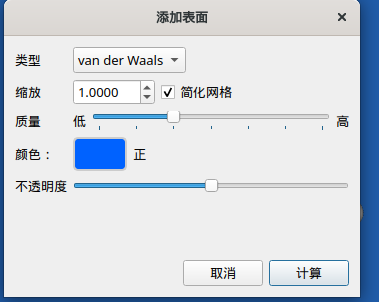
\includegraphics[scale=0.4]{figures/AddSurface.png}
\caption{用于 cube 数据文件的"添加表面"对话框}
\label{fig:cubefile}
\end{center}
\end{figure}

Cube 文件数据也可用于对表面着色。这将需要两个 cube 文件（一个包含表面数据，第二个包含用于对表面着色的
属性），或者一个 cube 文件和一个检查点文件。无论哪种情况，都需要使用上述文件 \bt\ 打开目录菜单项将两个文件
加载到同一个分子中。

创建表面后，双击表面项会弹出"配置表面"对话框：
\begin{figure}[h]
\begin{center}

\includegraphics[scale=0.15]{figures/SurfaceConfigurator.png}
\caption{"配置表面"对话框，将 Cube 数据显示为属性的一个选项。}
\label{fig:surfaceconfig}
\end{center}
\end{figure}

"属性"组合框将把 cube 数据作为选项之一，选择此项将使表面根据 cube 文件中的数据进行着色。可以通过单击
渐变框内部来更改渐变颜色。
\begin{figure}[h]
\begin{center}
\includegraphics[scale=0.30]{figures/ESP.png}
\end{center}
\caption{根据静电势着色的苯胺电子密度图。}
\end{figure}


\newpage
\subsection{轨道动画}

可以创建轨道动画 \eg{}，用于观看反应过程中前线轨道的演变，或观看自洽场（SCF）计算过程中轨道的弛豫。
关键帧应作为 cube 文件数据保存在单个目录中。cube 文件的基名需要与目录名匹配，\eg{}

\begin{center}
\hspace*{2em}{\tt  relaxation/relaxation.Frame.1.cube}\\
\hspace*{2em}{\tt  relaxation/relaxation.Frame.2.cube}\\
\end{center}
如第 \ref{sec:anal} 节所述打开目录，并右键单击模型视图中出现的第一个 cube 文件项，这将允许您访问
表面动画器对话框：
\begin{center}
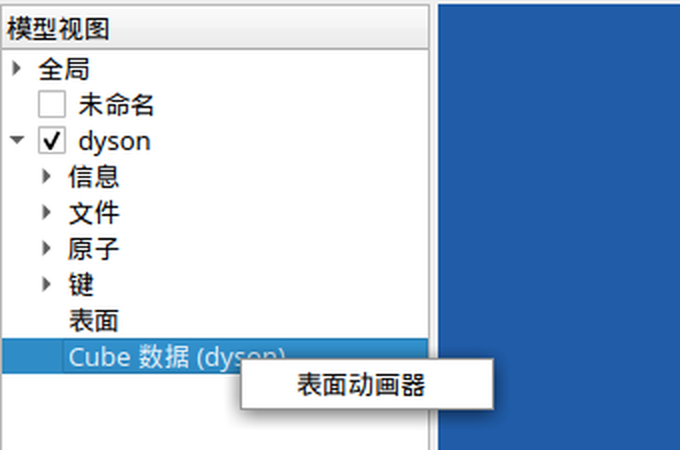
\includegraphics[scale=0.40]{figures/SurfaceAnimationMenu.png}
\end{center}
该对话框如图 \ref{fig:SurfaceAnimationDialog} 所示，可用于调整关键帧顺序和动画设置，包括插值帧数
（值越高结果越平滑，但耗时越长）。按 \Ovalbox{计算} 会生成每一帧，各个帧可以在模型视图中访问。使用
播放选项运行动画，并在需要时通过 \includegraphics[scale=0.40]{figures/RecordButton.png} 按钮录制动画。


\begin{figure}[h]
\begin{center}
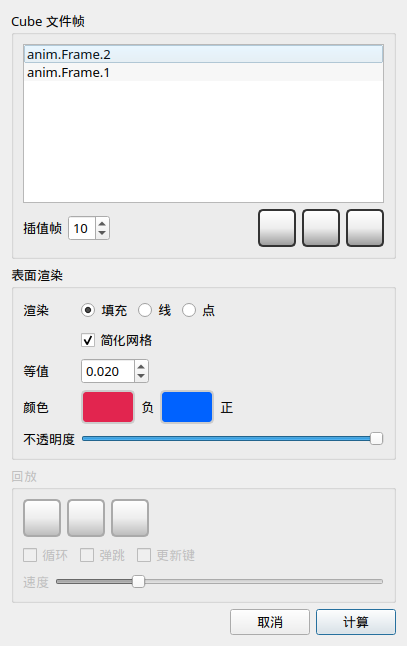
\includegraphics[scale=0.20]{figures/AnimationDialog.png}
\end{center}
\caption{表面动画对话框。}
\label{fig:SurfaceAnimationDialog}
\end{figure}



\newpage
\subsection{势能面}

几种计算类型提供有关势能面（PES）的信息。这些包括几何优化、势能面扫描、反应路径和过渡态搜索。打开包含
这些作业类型之一的 \qchem{} 输出文件时，模型视图中会出现一个"几何结构"项，双击它可以弹出"几何结构"对话框。
\begin{figure}[h]
\begin{center}
\includegraphics[scale=0.35]{figures/PesScan.png}
\caption{"几何结构"对话框，显示所选几何结构。}
\end{center}
\end{figure}

可以使用播放按钮在查看器中动画演示该路径，并且可以从表格中选择单个帧，或通过选择能量图上的一个点来选择。
查看器窗口将自动更新为相应的结构。与分子轨道能量图一样，能量图也可以缩放和滚动。

也可以从 XYZ 文件读入路径。其格式只是常规 XYZ 文件的拼接：
{\footnotesize
\begin{verbatim}
5
-291.77177
Si  0.71979   -0.08082   -0.76577
H   0.73262   -1.27801    0.22990
H   1.10451    0.93673    0.34825
H  -1.32980    0.23894   -0.28240
H  -1.22713    0.18317    0.47002
5
-291.76961
Si  0.67218   -0.07483   -0.72935
H   0.73053   -1.29428    0.22634
H   1.10815    0.95270    0.34714
H  -1.29502    0.23567   -0.33016
H  -1.19409    0.17584    0.49156
....
\end{verbatim}
}
第一行给出原子数，第二行（注释行）必须具有相应的能量，然后后面的行包含系统中每个原子的 xyz 坐标。
此模式对您拥有的任意多帧重复。


\subsection{振动频率}

可以从 \qchem{} 输出文件读入振动频率，并作为模型视图中的"频率"项出现。可以通过选择模型视图中关联的频率项
来可视化简正模式向量。
\begin{figure}[h]
\begin{center}
\includegraphics[scale=0.23]{figures/VibMode.png}
\caption{指示乙酸中简正模式的箭头。}
\end{center}
\end{figure}

双击模型视图中的频率会使分子根据所选模式振动。双击模型视图中的"频率"项会弹出振动频率对话框：
\begin{figure}[h]
\begin{center}
\includegraphics[scale=0.40]{figures/Frequencies.png}
\caption{振动频率对话框。}
\end{center}
\end{figure}

此对话框包含一个脉冲谱，显示频率的位置和相对强度。可以通过单击空心圆在谱上选择单个模式，这也会用所选模式
更新查看器窗口。可以使用高斯函数或洛伦兹函数加宽脉冲，以获得更逼真的谱，并且可以通过右键单击谱来弹出上下文
菜单导出图像。

谱的水平刻度可以缩放（使用鼠标滚轮）和平移（左键单击并拖动）以显示更多细节。

\subsubsection{同位素取代}

\iqmol{} 可以轻松地为 \qchem{} 振动频率计算设置同位素取代循环。首先在查看器中选择要取代的原子，然后选择
构建 \bt\ 设置同位素菜单项。将弹出一个对话框，允许您更改所选原子的同位素，以及更改用于计算热化学数据的
压力和温度。
\begin{figure}[h]
\begin{center}

\includegraphics[scale=0.20]{figures/IsotopeDialog.png}
\caption{同位素取代对话框，允许为所选原子指定非默认质量。请注意，每种元素类型只允许一个非默认质量。}
\end{center}
\end{figure}
选择质量后，单击确定，模型视图中会出现一个包含取代信息的"同位素"项。可以通过双击模型视图中相应的取代项来
编辑或检查它。可以通过在查看器中选择不同的原子和/或不同的质量来设置不同的取代，这些将在 \qchem{} 频率计算中
循环遍历。每个取代循环只需要在对角化之前对 Hessian 矩阵重新加权，因此一旦计算出 Hessian 矩阵，就可以非常
快速地获得多个循环。


\subsection{NMR 谱}

可以使用 \iqmol{} 可视化 NMR 屏蔽常数和化学位移。必须首先运行 \qchem{} 计算（JOB\_TYPE = NMR）并将输出文件
加载到 \iqmol{} 中。可以通过选择显示 \bt\ 原子标签 \bt\ NMR 选项，在查看器中将屏蔽常数显示为原子标签。
\begin{figure}[h]
\begin{center}
\includegraphics[scale=0.20]{figures/NmrDisplay.png}
\caption{显示 NMR 屏蔽常数的丙醇。}
\end{center}
\end{figure}

模型视图中会出现一个 NMR 项，双击此项会弹出 NMR 谱对话框。
\begin{figure}[h]
\begin{center}

\includegraphics[scale=0.35]{figures/NmrConfigurator.png}
\caption{NMR 谱对话框}
\end{center}
\end{figure}

可以显示各种谱（$^1$H、$^{13}$C 等），如果给定理论水平下有参考（\eg\ TMS），也可以显示化学位移。在表格中选择
行还会突出显示查看器中相应的原子，以便于识别。如果绘制了脉冲，则也可以选择这些脉冲来识别哪些原子负责所选信号。

与振动频率谱一样，可以通过右键单击图像弹出上下文菜单来导出 NMR 谱。


%----------------------------------------------------------------------%
\newpage
\section{外观}
%----------------------------------------------------------------------%

\subsection{查看器相机}

查看分子时，原子和表面的坐标固定在世界参考系中。当使用鼠标操纵分子时（见 \S\ \ref{sec:mousemodes}），实际上是
相机改变了位置和方向。如果需要更精确地控制相机（\eg\ 用于复现特定图像），则可以通过显示 \bt\ 相机菜单项配置
相机。默认情况下，相机使用透视投影以获得更好的深度感知，但也可以根据需要选择正交投影。

\begin{figure}[h]
\begin{center}

\includegraphics[scale=0.25]{figures/CameraDialog.png}
\caption{"配置相机"对话框允许精确控制查看器相机的位置和方向。}
\end{center}
\end{figure}



\subsection{裁剪平面}

提供了一个全局裁剪平面，可以通过在模型视图中启用全局下的"裁剪平面"项来查看。裁剪平面可用于显示表面信息而
不遮挡底层的分子结构。选择时，可以使用 \S\ \ref{sec:mousemodes} 中描述的操纵选择模式任意平移和旋转裁剪平面。
或者，可以通过双击模型视图中的"裁剪平面"项打开配置对话框来设置裁剪平面的精确方向。

\begin{figure}[h]
\begin{center}
\includegraphics[scale=0.30]{figures/ClippingPlane.png}
\caption{显示裁剪后的密度表面，使底层分子结构更容易看清的图像。}
\end{center}
\end{figure}

可以通过选择每个表面的表面配置器对话框（见图~\ref{fig:surfaceconfig}）中的"裁剪"复选框来裁剪各个表面。一旦
表面被裁剪，即使通过取消勾选模型视图中的"裁剪平面"项复选框将其隐藏，裁剪平面仍保持活动状态。


\subsection{着色器}

\iqmol{} 使用 GLSL 着色器来增强查看器的外观。可以通过显示 \bt\ 外观菜单项并选择"着色器"面板来激活着色器。
\begin{figure}[h]
\begin{center}

\includegraphics[scale=0.20]{figures/ShaderDialog.png}
\caption{配置着色器选项}
\end{center}
\end{figure}

对各种着色器选项的更改将立即生效，并且可以通过单击 \Ovalbox{另存为默认} 保存为默认值。某些着色器具有多个关联的
光源，可以打开或关闭这些光源以获得不同的光照效果。


\subsection{导出 POV-Ray 文件}

\iqmol{} 可以生成用于外部 POV-Ray 程序包的场景文件（.pov）。POV-Ray 使用光线追踪算法生成非常高质量和分辨率的
图像。POV-Ray 是开源的，但存在多个带有预编译二进制的官方和非官方程序包，特别是使用 Mac 版本的 MegaPOV 进行了
测试。二进制文件可从以下站点下载：
\begin{itemize}
\itemsep0em
\item Mac: \url{http://megapov.inetart.net/povrayunofficial_mac}
\item Windows: \url{http://www.povray.org/download}
\end{itemize}

要导出场景文件，请使用编辑 \bt\ 生成 POV-Ray 输入菜单项。场景文件是纯文本，包含供 POV-Ray 程序使用的指令，用户
可以在处理之前对其进行微调。\iqmol{} 可以对分子应用多种效果（\eg\ 表面纹理），这些可以通过打开外观对话框
（显示 \bt\ 外观菜单项）进行配置。

\begin{figure}[h]
\begin{center}
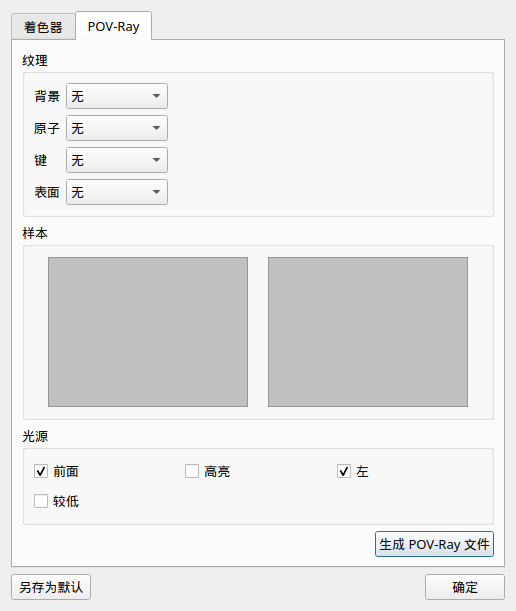
\includegraphics[scale=0.20]{figures/POVRayDialog.png}
\caption{外观对话框，显示 POV-Ray 场景文件的选项。}
\end{center}
\end{figure}

请注意，\iqmol{} 试图生成与查看器窗口中显示的内容尽可能匹配的场景文件。但是，光照、颜色和相机角度可能会有轻微
差异，可能需要一些反复尝试才能获得令人满意的图像。特别是，可能需要尝试 Gamma 值，并且根据为场景选择的是浅色
还是深色背景，可能需要更改环境光和漫反射光照（通过着色器选项）。


%----------------------------------------------------------------------%
\newpage
\section{示例图像}
%----------------------------------------------------------------------%

以下是一些可以使用 \iqmol{} 的着色器和渲染选项生成的图像示例。其中大多数只是屏幕截图，但是中间行的图块 3、4 和 5
是通过在 \iqmol{} 生成的场景文件上运行 POV-Ray 获得的。

\begin{center}
\includegraphics[scale=0.58]{figures/gallery/g13_sm.png}\
\includegraphics[scale=0.58]{figures/gallery/g14_sm.png}\
\includegraphics[scale=0.58]{figures/gallery/g15_sm.png}\
\includegraphics[scale=0.58]{figures/gallery/g16_sm.png}\
\includegraphics[scale=0.58]{figures/gallery/g21_sm.png} \\
\includegraphics[scale=0.58]{figures/gallery/g10_sm.png}\
\includegraphics[scale=0.58]{figures/gallery/g11_sm.png}\
\includegraphics[scale=0.58]{figures/gallery/g12_sm.png}\
\includegraphics[scale=0.58]{figures/gallery/g17_sm.png}\
\includegraphics[scale=0.58]{figures/gallery/g25_sm.png} \\
\includegraphics[scale=0.58]{figures/gallery/g1_sm.png}\
\includegraphics[scale=0.58]{figures/gallery/g4_sm.png}\
\includegraphics[scale=0.58]{figures/gallery/g23_sm.png}\
\includegraphics[scale=0.58]{figures/gallery/g26_sm.png}
\includegraphics[scale=0.58]{figures/gallery/g24_sm.png} \\
\includegraphics[scale=0.58]{figures/gallery/g7_sm.png}\
\includegraphics[scale=0.58]{figures/gallery/g5_sm.png}\
\includegraphics[scale=0.58]{figures/gallery/g3_sm.png}\
\includegraphics[scale=0.58]{figures/gallery/g20_sm.png}\
\includegraphics[scale=0.58]{figures/gallery/g18_sm.png} \\
\includegraphics[scale=0.58]{figures/gallery/g2_sm.png}\
\includegraphics[scale=0.58]{figures/gallery/g9_sm.png}\
\includegraphics[scale=0.58]{figures/gallery/g8_sm.png}\
\includegraphics[scale=0.58]{figures/gallery/g18_sm.png}\
\includegraphics[scale=0.58]{figures/gallery/g19_sm.png}\
\end{center}


%----------------------------------------------------------------------%
\newpage
\section{反应路径}
\label{sec:reaction}

如第 \ref{sec:anal} 节所述，几何优化、势能面扫描、过渡态搜索等作业会在模型视图中生成一个"几何结构"
项，其中包含了沿反应坐标的一系列结构帧。反应路径正是对这些帧进行连续播放所形成的动画。

要查看反应路径，请在模型视图中双击"几何结构"项，打开几何结构对话框（见图~\ref{fig:Pes}）。对话框
中央的能量图以曲线形式展示了各帧的相对能量，横轴为反应坐标，纵轴为能量。您可以通过以下方式与路径
交互：

\begin{itemize}
\item {\bf 播放/暂停：} 单击对话框中的播放按钮，即可在查看器窗口中连续播放沿反应坐标演化的结构动画。
\item {\bf 选择单帧：} 在能量图上单击某个数据点，或在下方的表格中选中某一行，查看器会立即更新为该帧对应
      的几何结构。能量值会显示在图表下方。
\item {\bf 缩放与平移：} 与分子轨道能级图类似，能量图可以使用鼠标滚轮缩放、左键拖动平移，以便查看局部细节。
\end{itemize}

\begin{figure}[h]
\begin{center}
\includegraphics[scale=0.35]{figures/PesScan.png}
\caption{几何结构对话框，显示所选的一帧几何结构及其在能量图上的位置。}
\label{fig:Pes}
\end{center}
\end{figure}

如果反应的能量曲线较为复杂（例如存在多个中间体），建议先在 QUI 中将作业类型设置为过渡态搜索或
势能面扫描，确保结果包含足够密集的帧，以获得平滑的路径动画。

路径数据也可以从外部的 XYZ 文件读入。该文件的格式为多个标准 XYZ 文件的顺序拼接：每一段的第一行为
原子数，第二行（注释行）必须给出该帧对应的能量，随后是各原子的 xyz 坐标。此模式可重复任意多帧。


\section{制作电影}
\label{sec:movie}

\iqmol{} 可以将查看器窗口中显示的连续画面录制为电影文件，便于在演示或论文中展示分子动画（例如反应路径、
轨道演化或振动模式）。录制功能由快照管理器（Snapshot）负责，支持将一系列帧合成为常见的视频格式。

制作电影的一般流程如下：

\begin{enumerate}
\item {\bf 准备动画场景：} 先在查看器中设置好要展示的动画，例如播放一条反应路径（见第 \ref{sec:reaction} 节）、
      轨道动画（见第 \ref{sec:anal} 节"轨道动画"）或振动模式。
\item {\bf 开始录制：} 单击查看器工具栏中的录制按钮
      \includegraphics[scale=0.40]{figures/RecordButton.png}
      开始捕获画面。录制期间对查看器的所有操作都会被记录。
\item {\bf 结束并生成：} 再次单击录制按钮停止录制。\iqmol{} 会调用外部工具（如 ffmpeg）将捕获的帧合成为
      电影文件。生成进度可在状态栏或日志中查看，完成后会提示电影文件已保存的位置。
\end{enumerate}

需要注意以下几点：
\begin{itemize}
\item 录制的电影质量取决于录制时的查看器窗口分辨率与渲染设置。如希望获得高分辨率影片，建议先在显示 \bt\
      外观菜单中调高渲染质量，或导出 POV-Ray 场景文件（见上一节）后用光线追踪渲染单帧再合成。
\item 合成电影依赖系统中已安装的视频编码器。若录制后未能生成文件，请检查是否已安装 ffmpeg 等工具，并确认
      其位于系统的可执行路径（PATH）中。
\item 对于需要精确控制每一帧的场景（如反应路径电影），更稳妥的做法是先将各关键帧导出为 cube 文件，再使用
      表面动画器（第 \ref{sec:anal} 节）生成插值帧，最后逐帧录制。
\end{itemize}


\section{配置}
\label{sec:config}

\iqmol{} 的大部分全局行为都可以通过"全局"项与首选项进行配置。模型视图（MV）中的"全局"（Global）项始终可用，
展开后可以看到外观、表面默认值、服务器列表等子项，双击即可进入相应的配置界面。

\subsection*{首选项}

选择编辑 \bt\ 首选项菜单项，或在模型视图中展开"全局"项并双击"首选项"，会打开首选项浏览器。其中常用的设置包括：

\begin{itemize}
\item {\bf 默认力场：} 设置分子力学优化的默认力场（默认通用力场 UFF）。可在构建 \bt\ 选择力场菜单中临时更改，
      此处为永久默认值。
\item {\bf 撤销步数上限：} 限制历史面板中可撤销操作的数量，避免占用过多内存。
\item {\bf 模型视图显示：} 控制程序启动时是否显示模型视图面板，以及主窗口的默认尺寸。
\item {\bf 任务监视器列表：} 记录以往提交作业的信息，可在计算 \bt\ 任务监视器中访问；选择"清除作业"可将其清空。
\end{itemize}

\subsection*{外观配置}

全局外观（背景颜色、着色器、裁剪平面等）通过显示 \bt\ 外观菜单项配置，相关内容已在本手册"外观"一章中
详细说明。将某项着色器选项改为满意效果后，可单击 \Ovalbox{另存为默认} 使其对所有后续分子生效。

\subsection*{服务器配置}

用于 \qchem{} 计算的本地或远程服务器在全局"服务器"项下统一管理。添加、编辑服务器的方法见"运行 Q-Chem 计算"
一章中的"配置服务器"一节。配置好的服务器列表会被保存，下次启动 \iqmol{} 时自动加载。

通过合理使用以上配置，可以将 \iqmol{} 调整为符合个人习惯的工作环境，并保持不同会话之间的一致性。


%----------------------------------------------------------------------%
\bibliographystyle{acm}
\bibliography{IQmolUserGuide}
%----------------------------------------------------------------------%

\end{document}
%----------------------------------------------------------------------%
